Consider a pair of nested ellipses $\mathcal{D}\subset \mathcal{C}$ as shown in \cref{fig:poncelet}. Let $P_0\in \mathcal{C}$ and draw a tangent line $L_1$ to $\mathcal{D}$ and passing through $P_0$. Call $P_1$ the second intersection of $L_1$ with $\mathcal{C}.$
From $P_1$ draw the the second tangent line $L_2$ to $\mathcal{D}.$
Clearly this process can be iterated to order $n. $
The sequence of points $\{P_0,P_1,P_2,\ldots, P_n,\ldots\}$ will be called the {\em Poncelet orbit}.

When $P_n=P_0$ the Poncelet orbit is called periodic and the polygon $\mathcal{P}_n$ with vertices $\{P_0,\ldots, P_{n-1}, P_n\}$ will be called an $n-$gon. So, we obtain a polygon interscribed in the pair of ellipses $\{\mathcal{D},\mathcal{C}\}.$

\begin{theorem}  Consider a pair of nested ellipses $\{\mathcal{D},\mathcal{C}\}$ as shown in \cref{fig:poncelet}. If there is a $n-gon$ interscribed between the pair $\mathcal{D}$ and $\mathcal{C}$, then for every $Q_1\in \mathcal{C}$ there is an $n-$gon interscribed between $\mathcal{D}$ and $\mathcal{C}$ having $Q_1$ as one of its vertices.

\label{th:poncelet}
\end{theorem}


\begin{figure}
\begin{center}
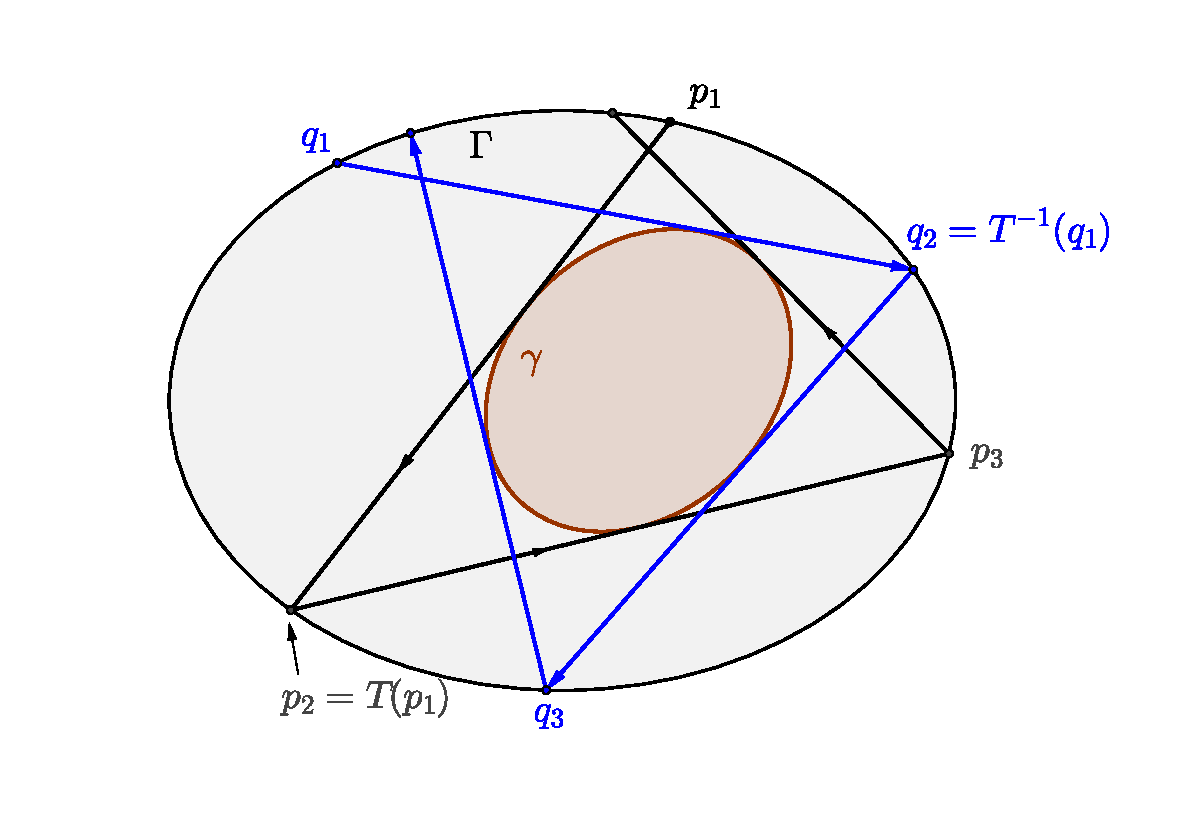
\includegraphics[scale=0.6]{chap_02/pics/pics_chap2-030-poncelet-map.pdf}
\end{center}
\caption{Poncelet map associated to the pair of ellipses $\{\mathcal{C},\mathcal{D}\}.$}
\label{fig:poncelet}
\end{figure}

The classical Poncelet theorem is about a natural generalization of billiards. Consider a pair of nested ellipses $\Gamma$ (outer) and $\gamma$ (inner) oriented by the external normal vector.
Consider a point $p\in \gamma$ and  $\ell_p$ the   tangent line  to $\gamma$ at $p$. Let $p_1$ and $p_2$ the intersection of  $\ell_p$ with $\Gamma.$ The Poncelet map is induced by the correspondence
$P_p:\Gamma\to\Gamma$, $P_p(p_1)=p_2$. Through $p_2$ consider the other tangent line to $\gamma$ and let $p_3$ the intersection of this line with $\Gamma$. Therefore, fixed a orientation we have a well defined map $T:\Gamma\to \Gamma$ with $T(p_1)=p_2,$ $T(p_2)=p_3$, etc. 
Changing the orientation is defined the inverse $T^{-1}.$ See  \cref{fig:poncelet}.

\begin{figure}[H]
	\begin{center}
	%	\def\svgwidth{1.0\textwidth}
	%	\input{pics_tex/poncelet_nested.pdf_tex}
	 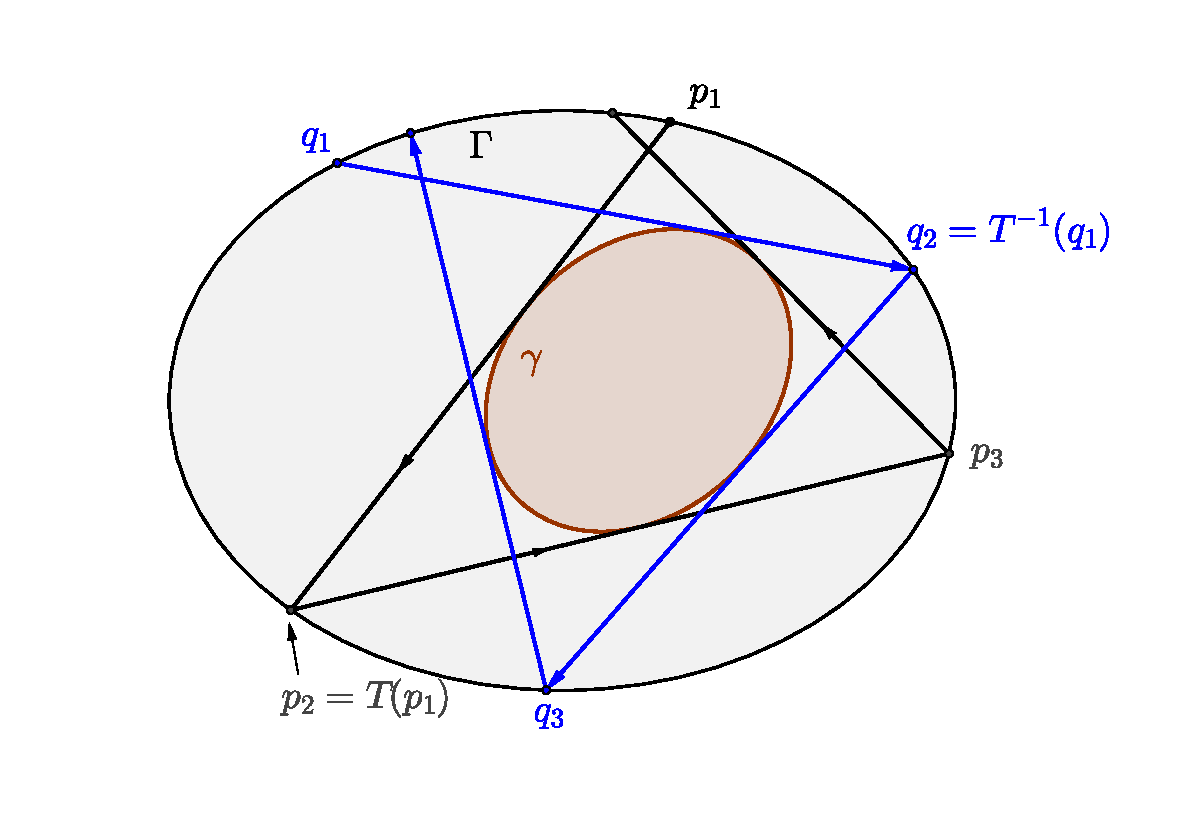
\includegraphics[scale=0.5]{chap_02/pics/pics_chap2-030-poncelet-map.pdf}
		\caption {Poncelet map  $T:\Gamma\to\Gamma$ with $T(p_1)=p_2$ and $T^{-1}:\Gamma\to\Gamma$ with $T^{-1}(q_1)=q_2$ associated to  a pair of nested ellipses $\gamma\subset\Gamma$.
		\label{fig:poncelet-map}}
	\end{center}
\end{figure}

The orbit of a point $p_1\in \Gamma$ is the polygon defined by the vertices $T^k(p_1)=p_k.$ 
A orbit of a point $p_1$ is called $N$-periodic when $T^N(p_1)=p_1.$ The $N$-gon is inscribed in $\Gamma$
and circumscribed about $\gamma.$
The Poncelet theorem is following.
\begin{theorem}[Poncelet's Closure Theorem] Consider a pair of nested ellipses $\gamma\subset \Gamma$. If $T:\Gamma\to\Gamma$ has a periodic orbit for some $p_1$ then all orbits are periodic. 
\end{theorem}
%
For a historical and proofs of this theorem see \cite{barth1996}, \cite{centina2016a}, \cite{centina2016b}, \cite{chasles1843}, \cite{drag2014} and references therein. See also    \cite[Chapter IV]{berger2010},  \cite{cima2010},\cite{cieslak2016}, \cite[Livre III, Chapitres II, III]{darboux1917}, \cite{drag_milena2011},  \cite[Chapter 9]{gla2016}, \cite{hahu2015}, \cite{hahu2017}, \cite{leb1921},  \cite{mirman2012},  \cite{poncelet1822} and \cite{previ1999}.

The proof presented below  is based in \cite{shoe1983}. 
Consider an ellipse and a circle given by
\[\mathcal{E}_{a,b}: \;\frac{x^2}{a^2}+\frac{y^2}{b^2}=1, \;\;\; \mathcal{C}_r:\; x^2+y^2=r^2, \; 0<r<b<a.\]

For the reduction of a general pair of nested ellipses to the pair above and a proof of Poncelet's Porism theorem   see \cite{bry}.

Let $P=(a\cos\varphi, b\sin\varphi)$ and $P'=(a\cos\varphi, a\sin\varphi)$ as shown in   \cref{fig:ec}.
\begin{figure}[H]
	\begin{center}
	%	\def\svgwidth{0.8\textwidth}
	%	\input{pics_tex/poncelet_elipse_circulo.pdf_tex}
		 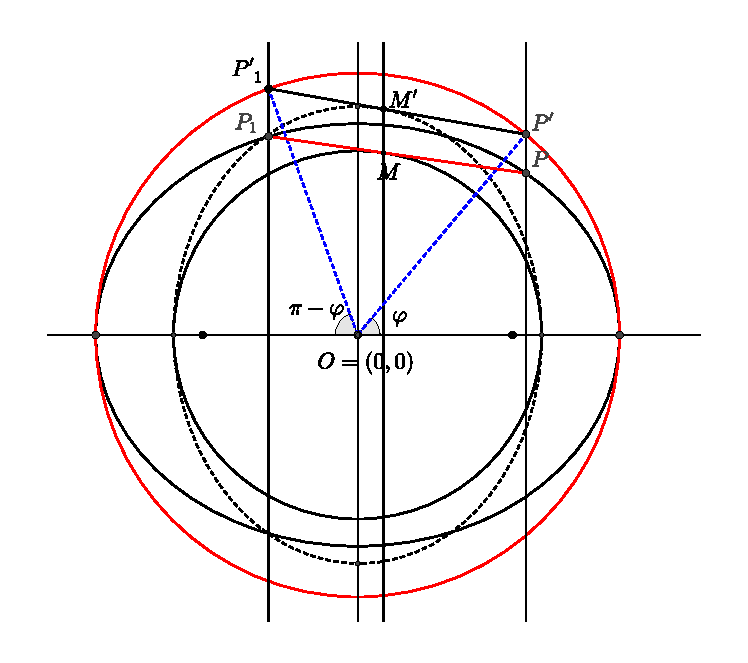
\includegraphics[angle=0, width=12cm]{chap_02/pics/pics_chap2-010-poncelet-proof.pdf}
		\caption { Poncelet maps $T:\mathcal{E}_{a,b}\to\mathcal{E}_{a,b}$ with $T(P)=P_1$ and $T:\mathcal{C}_{a}\to\mathcal{C}_{a}$ with $T'(P')=P_1'$ associated to  the pairs $\{\mathcal{E}_{a,b},\mathcal{C}_r\}$ and $\{\mathcal{C}_a,\mathcal{E}_{r,ra/b}\}$. \label{fig:ec}}
	\end{center}
\end{figure}
Consider the tangent line $PP_1$ to $\mathcal{C}_r$ at the point $M$, and let
\[\angle AOP'=\varphi, \;\; \angle AOP_1'=\varphi_1.\]
\begin{proposition} In the above conditions it follows that:
    \begin{equation}
        \left(\frac{d\varphi_1}{d\varphi}\right)^2=\frac{1-k^2\sin^2\varphi_1}{1-k^2\sin^2\varphi}
            \label{eq:variacaoangular}
    \end{equation}
    \label{prop:variacaoangular}
\end{proposition}
 \begin{proof}
 Let $A(x,y)=(x,\frac{b }{a} y)$ be the affine transformation sending the circle $\mathcal{C}_a$ of radius $a$ to the ellipse $\mathcal{E}_{a,b}.$ Define the points $M'=T^{-1}M$ and $P_1'=T^{-1}{(P_1)}$. The envelope of the family of  lines $P'P_1'$ is an ellipse $\mathcal{E}_{r,ar/b}$ of semiaxes $r$ and $\frac{ar}{b}>r$ wich is tangent to $M_1'$. See  \cref{fig:ec}. 
 
 The line $P'M'P_1'$ intersects the circle $\mathcal{C}_a$ in equal angles, and it follows that
 \[\frac{d\varphi_1}{d\varphi}=\frac{|M'P_1'|}{|M'P'|}=\frac{|MP_1|}{|MP|}.\]
    Now observe that
    \begin{align*}
    |MP|^2=&|OP|^2-|OM|^2 = a^2\cos^2\varphi+b^2\sin^2\varphi-r^2\\
    &=a^2-r^2-(a^2-b^2)\sin^2\varphi\\
    &=(a^2-r^2)\left(1-\frac{a^2-b^2}{a^2-r^2}\sin^2\varphi\right)\\
    &=(a^2-r^2)(1-k^2\sin^2\varphi),\;\;k^2=\frac{a^2-b^2}{a^2-r^2}<1.\\
     |MP_1|^2=&|OP_1|^2-|OM_1|^2=(a^2-r^2)\left(1-k^2\sin^2\varphi_1\right)
    \end{align*}
 \end{proof}
 
 \begin{proposition} Let 
 \[J(\varphi,\varphi_1)=\int_{\varphi}^{\varphi_1}\frac{dx}{\sqrt{1-k^2\sin^2x}}.\]
 Then $J(\varphi,\varphi_1) =\text{cte}$ is independent of the initial position $\varphi.$
     
 \end{proposition}
 
 \begin{proof} Follows directly from   \cref{eq:variacaoangular} and Fundamental Theorem of Calculus.
 \end{proof}
 \begin{remark} By the construction above it follows that
$A\circ T'=T\circ A$ and therefore the two billiard maps $t$ and $T'$ are conjugated by the affine map $A$.
\end{remark}
 
    \begin{theorem} [Poncelet] Consider the nested pair of an ellipse $ \mathcal{E}_{a,b}$ and a circle $\mathcal{C}_r$. Consider a polygonal orbit $\mathcal{P}_n=P_1P_2\ldots P_n$ inscribed in $\mathcal{E}_{a,b}$ and circumscribed about $\mathcal{C}_r$. If after one revolution along $ \mathcal{E}_{a,b}$ the polygon $\mathcal{P}_n$ is closed, then all orbits will be closed.
    
\end{theorem}

\begin{proof} Denote $P_k=(a\cos\varphi_k,b\sin\varphi_k)$ with $\varphi_0=\varphi.$ As $J(\varphi,\varphi_1)=\omega=\text{cte}$, it follows that for a n-periodic orbit with turning number $N$ we have
$J(\varphi,\varphi+2\pi N)= n\omega$. 
\end{proof}

